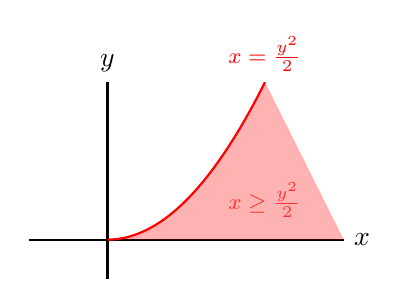
\begin{tikzpicture}
%Axis
\draw[thick] (-1,0)--(3,0) node[right]{$x$};
\draw[thick] (0,-0.5)--(0,2) node[above]{$y$};

\draw[thick, red, domain=0:2,samples=40] plot(\x,{\x^2 / 2}) node[above] {\footnotesize $x=\frac{y^2}{2}$};

\fill [red, opacity=0.3, domain=0:2, variable=\x]
      (0, 0)
      -- plot ({\x}, {\x^2 / 2})
      -- (3, 0)
      -- cycle;

\node[red, opacity=0.7] at (2,0.5) {\footnotesize $x \geq \frac{y^2}{2}$};

\end{tikzpicture}

